%*
%* Seven Kingdoms: Ancient Adversaries
%*
%* Copyright 1997,1998 Enlight Software Ltd.
%* Copyright 2018 Timothy Rink
%*
%* This program is free software: you can redistribute it and/or modify
%* it under the terms of the GNU General Public License as published by
%* the Free Software Foundation, either version 2 of the License, or
%* (at your option) any later version.
%*
%* This program is distributed in the hope that it will be useful,
%* but WITHOUT ANY WARRANTY; without even the implied warranty of
%* MERCHANTABILITY or FITNESS FOR A PARTICULAR PURPOSE.  See the
%* GNU General Public License for more details.
%*
%* You should have received a copy of the GNU General Public License
%* along with this program.  If not, see <http://www.gnu.org/licenses/>.
%*
%*

\chapter{Developing Your Economy}

\index{economic development}

\section{Mines and Their Placement}

\index{mines!placing}
\index{placing mines}

\begin{wrapfigure}{l}{0.3\textwidth}
    \vspace{-20pt}
    \begin{center}
        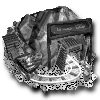
\includegraphics[width=0.3\textwidth]{Imine} % Original size.
        \\ Mine
    \end{center}
    \vspace{-30pt} % -30pt
\end{wrapfigure}

\textgoth{\Huge{M}}ines are required if your Empire is to have an assured source of raw materials. Although it is possible to prosper through trade, this may force you into a dependent relationship with other kingdoms.

All Mines must be built by a unit trained in either Mining or Construction atop a Natural Resource deposit. \\ %

\subsection{Natural Resources}

\index{natural resources}

% add hspace

\begin{center}

\includegraphics[width=0.5\linewidth]{Iresources} % Original size.
\\ Copper Iron Clay
\end{center}

\textgoth{\Huge{S}}cattered across the world, you will find the Natural Resources pictured above. \textbf{Clicking} on any of these icons will reveal its type and the amount of the Resource deposit.

% Hyphenation here. Key here.

On the small World Map, these Natural Resources will appear as a small black square. These are more easily seen in the middle or right hand modes of the World Map screen. The ‘J’ hot-key may also be used to quickly locate Resources.

\subsection{Building Your Mines}

\index{building!mines}
\index{mines!building}

\begin{wrapfigure}{r}{0.1\textwidth}
    \vspace{-20pt}
    \begin{center}
        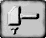
\includegraphics[width=0.1\textwidth]{Thammer}
    \end{center}
    \vspace{-20pt}
\end{wrapfigure}

% Bold Cursor?

\textgoth{\Huge{T}}o build a Mine, send a unit trained in either Mining or Construction to the site of the Natural Resource. \textbf{Click} on the \textbf{Construction Tile} and then choose Build Mine. Center the flashing square and Construction Cursor over the Natural Resource and \textbf{Click}. The Mine will then be built on that spot.

The Mine, once built, cannot begin operations until workers, preferably trained in Mining, are assigned to it. If the Mine was built by a unit trained in Mining, he will automatically be assigned there.

Over time, the skill level of the workers will increase. This will directly affect their output. A Mine with one worker with a skill level of 80 will have the same output as a Mine with four workers with skill levels of 20 each.

\subsection{Linking Your Mines}

\index{linking mines}
\index{mines!linking}

\textgoth{\Huge{I}}f the Mine is Linked to a Village and the Link is open, Peasants from the Village will voluntarily go to work down in the pit as even Mining is better than being a Peasant. If there are not enough Peasants in the Village or if the Mine is beyond Linking range with any Village, you may Recruit and assign with a \textbf{Right-Click} either Peasants or trained Miners to it.

Since most of the time, those Natural Resources will be far removed from your Villages and therefore out of direct Linking range. Transportation of the mined materials to one of your Factories or Markets must be taken care of by way of a Caravan.

\textbf{NOTE}: When a new Mine, or other building with workers, is built out of direct Linking distance of a Village, the workers will settle a new Village next to their place of work. Although this new Village will belong to you, you will not be able to fully control it unless you build a new Fort Linked to it.

If there is no place for a new Village to be settled, then you will be unable to assign anyone to work there.

% COMMA HERE

The above three Natural Resources are the only ones that you will find in this world. It is essential that you acquire at least one of them, either through Mining or Trade. Without them, you cannot operate Factories to produce Finished Goods and sell them for money.

\subsection{Operational Information}

\index{mines!operational information}

\begin{wrapfigure}{r}{0.4\textwidth}
    \vspace{-20pt}
    \begin{center}
        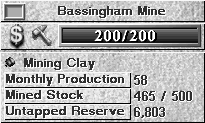
\includegraphics[width=0.4\textwidth]{Imineinfo} % Original size.
    \end{center}
    \vspace{-50pt}
\end{wrapfigure}

\textgoth{\Huge{W}}hen you \textbf{Click} on one of your Mines, you will be able to see, on the Right, all of the information about its operation. This includes:

\textbf{The Raw Material} being mined.

\textbf{The Monthly Production} output.

\textbf{The amount of Mined Stock} waiting for movement out of the Mine.

Mines can hold a maximum of 500 units of Mined Stock. If this limit is reached, all work will cease until a Caravan picks some up or a Direct Link is established with a Factory or a Market. If a Direct Link is established with a Harbor, the Raw Materials will remain in the Mine until a Ship of Trade Leaves the Harbor.

\textbf{The Untapped Reserve}: This shows you how much more Raw Material is left to be extracted from the mine.

\begin{center}
    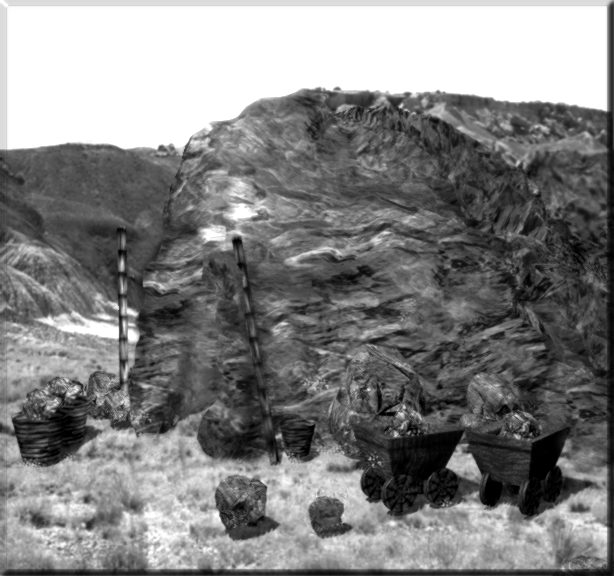
\includegraphics[width=0.6\linewidth]{Amine} % Original size.
\end{center}

\section{Factories and Finished Goods}

\begin{wrapfigure}{l}{0.3\textwidth}
    \vspace{-20pt}
    \begin{center}
        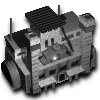
\includegraphics[width=0.3\textwidth]{Ifactory}
        \\ Factory
    \end{center}
    \vspace{-20pt}
\end{wrapfigure}

% Author's voice.

\textgoth{\Huge{F}}actories should be manned in the same way as Mines, except that an ideal Factory worker should be trained in Manufacturing. As with mines, a Factory built out of direct Linking distance from a Village will have to have workers assigned to it by you. They will then settle a new Village next to the Factory.

With the above raw materials available, the Factory will begin producing Finished Goods. It is the sale of these Finished Goods in markets around the world that generates the most money for your coffers.

\subsection{Finished Goods}

\index{factories!finished goods}

\begin{center}
    
\includegraphics[width=0.5\linewidth]{Igoods} % Original size.
    \\ Copperware Ingots Pottery
    \\ (Copper) (iron) (Clay)
\end{center}

\subsection{Toggling Production}

\index{factories!toggling production}
\index{toggling factory production}

\begin{wrapfigure}{r}{0.1\textwidth}
    \vspace{-20pt}
    \begin{center}
        
\includegraphics[width=0.1\textwidth]{Tgoodcycling}
    \end{center}
    \vspace{-20pt}
\end{wrapfigure}

% Parentheses here

\textgoth{\Huge{W}}hen the Factory is selected, \textbf{Click} on the \textbf{Production Tile} to toggle the items that you want produced in that Factory.

In order for the desired Finished Good to be produced in your Factory, you must have the appropriate kind of Raw Materials being delivered there.

Your Factory will automatically take in Raw Materials from a Linked Mine (which must be yours) or Market (which may belong to any kingdom with which you have a trade treaty).

\clearpage

\subsection{Operational Information}

\index{factories!operational information}

\begin{wrapfigure}{r}{0.4\textwidth}
    \vspace{-20pt}
    \begin{center}
        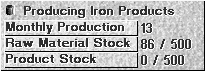
\includegraphics[width=0.4\textwidth]{Ifactoryinfo} % Original size.
    \end{center}
    \vspace{-20pt}
\end{wrapfigure}

\textgoth{\Huge{W}}hen you \textbf{Click} on one of your Factories, you will be able to see, on the Right, all of the information about its operation.

% See next comment below.

This information includes:

\textbf{Monthly Production}: quantity of Finished Goods being produced every month.

\textbf{Raw Material Stock}: quantity of Raw Material you have received from a Mine but have yet to convert into Finished Goods. If this reaches its maximum of 500, then you will be unable to receive any more Raw Materials.

% COMMA here

\textbf{Product Stock}: quantity of Finished Goods completed, but which have yet to be delivered to a Market or picked up directly from the Factory. If this number reaches the Maximum of 500, then production in your Factory will shut down until some of the units have been cleared.

\begin{center}
    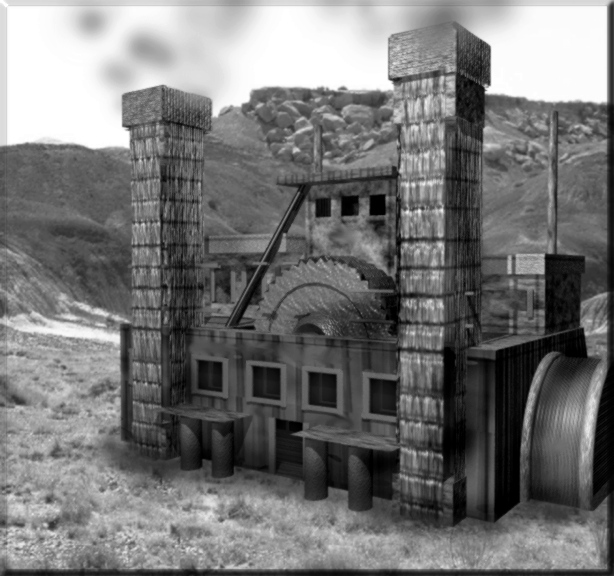
\includegraphics[width=0.45\linewidth]{Afactory} % Original size?
\end{center}

\clearpage

\section{Markets and Caravans}

\index{building!markets and caravans}

\subsection{Building and Linking Markets}

\index{markets!building}

\begin{wrapfigure}{l}{0.3\textwidth}
    \vspace{-20pt}
    \begin{center}
        
\includegraphics[width=0.3\textwidth]{Imarket} % Original size.
        \\ Market
    \end{center}
    \vspace{-30pt} % -30pt
\end{wrapfigure}

\index{caravans!building}

% Parentheses here

\textgoth{\Huge{A}}s was previously discussed, the correct use and placement of Markets is the key to a successful and profitable economy. As Markets are where your people buy and sell Raw Material and Finished Goods, they need to be Linked directly to Villages and Factories and, if you like, Mines (preferably all three at the same time). They may also be indirectly Linked to Mines, Factories, or other Markets by Caravans.

\begin{center}
    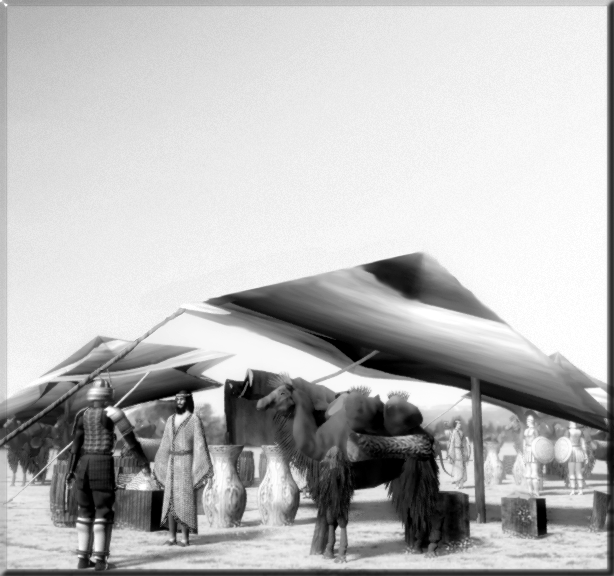
\includegraphics[width=0.7\linewidth]{Amarket} % Original size.
\end{center}

\clearpage

\subsection{Operational Information}

\index{markets!operational information}

\begin{wrapfigure}{r}{0.4\textwidth}
    \vspace{-20pt}
    \begin{center}
        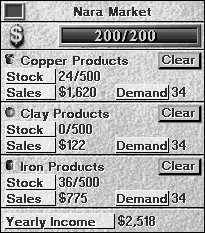
\includegraphics[width=0.4\textwidth]{Imarketinfo} % Original size.
    \end{center}
    \vspace{-20pt}
\end{wrapfigure}

\textgoth{\Huge{W}}hen you \textbf{Click} on one of your Markets, you will be able to see, on the Right, all of the information about its operation.

% I see three.

You will be able to see, after the name of the Market and its repair status, three rows of information on the three spaces available in the Market for the placement of goods. In this example, only two places have been filled.

In the row for Iron Products, you can see:

% this spot is interesting. added colons

\textbf{Stock}: how many units of Iron Ingots are on hand.

\textbf{Sales}: how much money you have made in the past 365 days from the sale of Iron Ingots.

\textbf{Demand}: whether or not you could be selling more if you produced more. An oversupply will also be obvious by the goods being stacked up in your Market.

In another row, you see much the same for Clay Products.

If you wish to clear a space in your Market for something else to be sold, \textbf{Click} on the \textbf{Clear Button}. That row will then be emptied of all goods.

\textbf{Yearly Income}: the total amount earned for all sales in this Market for the past 365 days.

\subsection{Hiring and Routing Caravans}

\begin{wrapfigure}{r}{0.1\textwidth}
    \vspace{-20pt}
    \begin{center}
        
\includegraphics[width=0.1\textwidth]{Tcamel} % Original size.
    \end{center}
    \vspace{-20pt}
\end{wrapfigure}

\index{caravans!hiring and routing}
\index{hiring and routing caravans}

\textgoth{\Huge{W}}hile the Market is selected, \textbf{Click} on the \textbf{Hire Caravan Tile}. A Camel will be hired and then stand outside your Market waiting for its assignment. To designate a route for your Caravan, you will be presented with the Caravan Routing area as seen on the right.

\subsubsection{How do I set the Caravan’s route?}

\begin{wrapfigure}{r}{0.4\textwidth}
    \vspace{-20pt}
    \begin{center}
        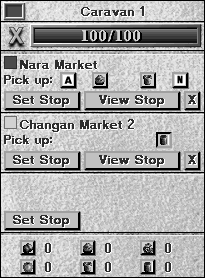
\includegraphics[width=0.4\textwidth]{Icamelinfo} % Original size.
    \end{center}
    \vspace{-20pt}
\end{wrapfigure}

Your Caravan will begin with one default stop. That is the Market at which it was hired. This may, of course, be changed.

You begin to set your Caravan’s routes by \textbf{Clicking} on the \textbf{Set Stop Button}.

% CURSOR here.

Your cursor will then change into the Camel and Arrow Cursor as seen below.


\includegraphics[width=0.2\linewidth]{Bcamel}

With this new cursor, \textbf{Click} on any other Market or at any of your Factories or Mines. Remember that this is only necessary if those Factories or Mines are beyond direct Linking distance of your Market.

You may not \textbf{Click} on a foreign Factory or Mine or on a foreign Market belonging to a Kingdom with which you do not have a Trade Treaty.

% INFORMAL

If you later want to see where a Caravan stop is, \textbf{Click} on the \textbf{View Stop Button} on the row of the stop you are interested in. Your main screen will then be centered over that stop.

If you want to clear a set stop, \textbf{Click} on the \textbf{X Button}. That stop will then be erased and the space left empty for another Set Stop.

\subsection{Setting Caravan’s Loads}

\index{caravans!setting loads}

\textgoth{\Huge{W}}hen a stop has been set, you will see on the same line all the possible loads that your Caravan may carry, depending upon what is available at that location.

% looks strange. , “Pick up:”.

To set your load, you must \textbf{Click} on the small buttons to the right of the words, “Pick up:”. For these buttons, you have the following choices:

\subsubsection{Automatic (A)}

% Not (A) ? FACTUAL?

\textbf{Click} on the \textbf{A}, and your Caravan will pick up goods if there are more than 100 units of those goods and if the supply is more than the demand.

\subsubsection{Nothing (N)}

\subsubsection{Why Would You Want to Set Nothing?}

% Contraction here.

For instance, let’s say that you want to pick up Raw Materials from a Mine, take them to a Factory, and then return empty to the Mine.

% Parentheses here

\begin{changemargin}{.5cm}{0cm}
In the first row, you would Set Stop at the Mine and then set the load to the Mine’s raw material. (You may also set Automatic.)

In the second row, you would Set Stop at the Factory, but as there would be nothing at the Factory that you would want to take back to the Mine, you would in that case set the load to (N). The Caravan will then go back empty to the Mine for another load of raw material.

% (N): Bold. Parentheses here

Instead of \textbf{Clicking} on (N), you may also deselect (button out) any icon that has been selected (button in).
\end{changemargin}

\textbf{NOTE}: If you set the first stop as the Factory and the second stop as the Mine, the resulting transfer of material would be the same.

\subsubsection{Raw Materials or Finished Goods}

\textbf{Click} on the small buttons of Raw Materials or Finished Goods that you wish to transport. You may \textbf{Click} on more than one if you wish.

% Quotations here

If your have set Help to “Detailed”, holding your cursor over one of the buttons will bring up the Help text. You will then be able to see which material is represented by the icon.

\subsubsection{Maximum Loads}

Your Caravans may carry a maximum of 100 units of each material. This may seem like a huge load for a single camel, but remember that the camel you see is symbolic of a Caravan, which is made up of a long train of camels.

\subsection{Can You Drop off Your Goods at Foreign Markets?}

\index{closed markets}

\textgoth{\Huge{N}}o. If you were allowed to do this, the builders of a Market would quickly lose control over what goods are being placed there. The Kingdom which owns the market is the only one who may sell goods there.

If you have a Trade Treaty with a foreign Kingdom, however, you may build your own Market in their territory, a Market that is Linked to their Villages and into which you may drop off your goods for sale to the people of that Kingdom.

\textbf{NOTE}: The Villagers of foreign Kingdoms will purchase goods from their own Markets before they purchase goods from yours, so if you are planning to build a Market in a foreign Kingdom, make sure that you put on sale only those goods that the locals do not already have access to or of which they have an insufficient supply.

\subsection{Closed Markets}

\index{markets!closed}

\textgoth{\Huge{S}}ome foreign Markets may be closed to your Caravans for political reasons. In this case, when you \textbf{Click} on a foreign Market, you will be notified that you may not trade here. In situations like this, it will become necessary for you to make a Trade Treaty with that Kingdom.

\subsection{Healing Injured Caravans}

\index{caravans!healing injured}

\textgoth{\Huge{I}}f you wish to heal an injured Caravan or to keep it out of a dangerous area, just delete one of its stops. The Caravan will then stop moving, and like any other unit that is at rest, it will heal itself. To start it moving again, just set a new second stop.

% Bold X ?

If the Caravan is severely injured, it may just be easier to disband it by \textbf{Clicking} on the X icon and then hire a new one.

\subsection{Limits on Caravan Numbers}

\index{caravans!limits}

\textgoth{\Huge{O}}ne Caravan needs ten Villagers to support it. If you have exceeded this limit, the \textbf{Hire Caravan Tile} will become disabled, and you will be unable to hire additional Caravans.

If you later have a drop in Villager population, you will not, however, lose your current Caravans.

\subsection{Attacking Caravans}

\index{caravans!attacking}
\index{attacking!caravans}

\textgoth{\Huge{Y}}ou may think it very clever to attack and destroy your opponent’s Caravans and thereby cripple that Kingdom's economy. You will soon learn, however, that the people of this world look upon this sort of behavior with horror. Do it if you must but in the certainty that your Reputation will be crippled for years to come.

\subsection{Disbanding Caravans}

\index{caravans!disbanding}
\index{disbanding caravans}

% X: I want this to be bold type. Hyphenation here.

\textgoth{\Huge{I}}f you wish to disband a Caravan, just \textbf{Click} on the big X to the left of the Hit-Point bar.

\section{Trading Situations}

\index{trading}

\textgoth{\Huge{A}}lthough you may find it distasteful to deal with the likes of common tradesmen, you will soon discover that Trade is the lifeblood of your Empire. Without Trade, you will be remembered as ruling the smallest and poorest Empire in history.

Below, you will find some of the most common Empire building situations, situations that call for expertise in Trading. The advice offered should be ignored at your peril.

In the charts to the right of the descriptions, the dark gray lines will represent direct Links. The dark gray lines with a Camel or a Trader will represent Caravan or Shipping Links.

\clearpage

\subsection{Situation A: You have a producing Mine. What do you do with the Raw Material?}

\begin{wrapfigure}{r}{0.4\textwidth}
    \vspace{-20pt}
    \begin{center}
        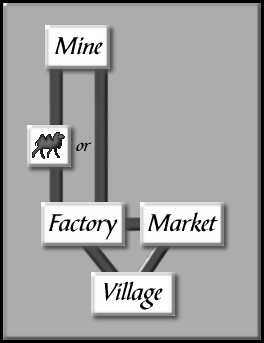
\includegraphics[width=0.4\textwidth]{Itradesit1} % Original size.
    \end{center}
    \vspace{-20pt}
\end{wrapfigure}

\textgoth{\Huge{Y}}ou must build a Factory that can make Finished Goods from those Raw Materials.

In order to receive the Raw Material, the Factory must be Linked, either directly or by Caravan, with the Mine.

% Parentheses here

In order to sell the Finished Goods (and to hire the Caravan), you must build a Market. Trade will be rendered more efficient if this Market is built close enough to be directly Linked to your Factory, while at the same time being close enough to be Linked to your Village. This is most important. Without that Link to a Village, you will be unable to sell Finished Goods.

Your profit in this situation will be \$4 per unit.

\clearpage

\subsection{Situation B: You have no mines, yet you wish to produce Finished Goods.}

\begin{wrapfigure}{r}{0.4\textwidth}
    \vspace{-20pt}
    \begin{center}
        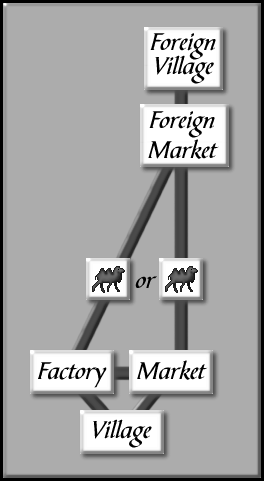
\includegraphics[width=0.4\textwidth]{Itradesit2} % Original size.
    \end{center}
    \vspace{-20pt}
\end{wrapfigure}

\textgoth{\Huge{Y}}ou must first build a Market and then hire a Caravan in that Market.

Next, look for a foreign Market that has Raw Materials available. You may not send your Caravan directly to a foreign Mine.

Send your Caravan to that Market, making sure that it is set to pick up the Raw Material that your want.

Your Caravan will go to that Market and return with a load of that Raw Material.

You may set the stop for that Caravan to return to as your Factory or your Market.

If you set the Market as the stop, your Caravan will drop off its goods there and then go back for another load. Your Factory will then take the Raw Materials from the Market and use them to produce the Finished Goods.

If you send the Caravan to the Factory, you will produce the Finished Goods as before, but you will leave one space free in your Market for other goods. For this reason, it is the preferred method.

After you produce and sell Finished Goods made from those Raw Materials, your profit will be \$3 per unit. The foreign Market will earn \$1 per unit from the sale of its Raw Materials.

\clearpage

\subsection{Situation C: In one Village, you have a lot of potential consumers, yet you have no Finished Goods to sell them and no chance to produce them yourself.}

\begin{wrapfigure}{r}{0.5\textwidth}
    \vspace{-20pt}
    \begin{center}
        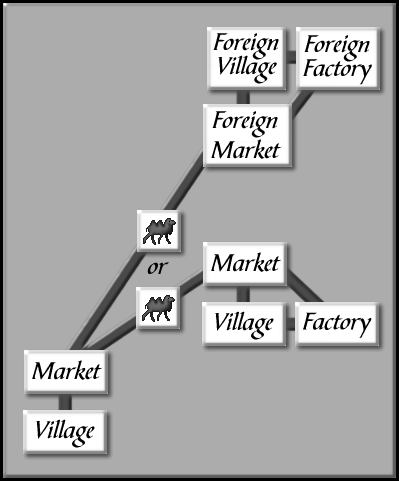
\includegraphics[width=0.5\textwidth]{Itradesit3} % Original size.
    \end{center}
    \vspace{-20pt}
\end{wrapfigure}

\textgoth{\Huge{F}}rom one of your Markets, hire a Caravan.

Next, send that Caravan to another of your Markets or to a foreign Market belonging to a Kingdom with which you have a Trade Treaty. You must, of course, look to make sure that that Market is selling Finished Goods.

Set your Caravan to pick up Finished Goods just as you picked up the Raw Material above.

When your Caravan returns, it will place those goods in its home Market for sale to your Villagers.

Your profit in this situation will be \$4 per unit if you are trading with another of your own Markets.

If you are trading with a foreign Market, your profit will be \$2 per unit. The foreign Market will also earn \$2.

\clearpage

\subsection{Situation D: You have many skilled Factory workers, turning out a surplus of goods.}

\begin{wrapfigure}{r}{0.5\textwidth}
    \vspace{-20pt}
    \begin{center}
        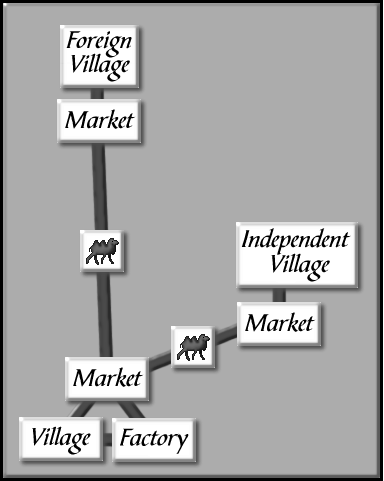
\includegraphics[width=0.5\textwidth]{Itradesit4} % Original size.
    \end{center}
    \vspace{-20pt}
\end{wrapfigure}

\textgoth{\Huge{A}}s a large amount of surplus goods sitting in your Market are doing you no good, the obvious solution is to either sell the goods abroad or move them to another of your Markets.

To do this, hire a Caravan, and then make sure that it is set to pick up that surplus from your Market.

Next, send that Caravan to one of your Markets that is Linked to another of your Villages, an independent Village, or to a Village belonging to a Friendly or Allied Kingdom.

Those goods will now be sold in the new Market. Remember that in order to sell to Independent Villagers, the average resistance level of the Village to your rule must be below 50.

Your profit in these situations will be \$4 per unit.

\textbf{NOTE}: You will be unable to build a Market Linked to a Village of another Kingdom unless your two Kingdoms have a Trade Treaty. You can check the Trade situation in the Kingdoms Scroll (F1).

\subsection{How can you sell even more goods in the above situation?}

\textgoth{\Huge{H}}aving a large population is the best bet to generate a lot of demand for goods. You will then be able to generate a lot of money, even if you never have a Mine, by importing Raw Materials or Finished Goods. It is important also to remember that people with jobs will spend more money than Peasants. If you bring jobs to your Villages or to Independent Villages, thus taking peasants out of the fields and giving them a salary, you will see your sales increase. This is because a Peasant will buy only six goods per year, while a salaried worker will buy 12 goods per year. These jobs are created with the building of Factories, Mines, Towers of Science, and War Factories.

Unlike your own workers, however, you must pay foreign workers \$10 per year. This should give you incentive to absorb their Villages by force or persuasion as soon as possible.

\subsection{Can other Kingdoms hire my workers?}

\textgoth{\Huge{Y}}es they can. If a Kingdom that has a trade treaty with you builds a firm Linked to one of your Villages, it may hire your workers. In this situation, they must pay \$10 per year into your treasury for each worker hired. An added advantage for you is that when you have a worker in another’s building, you will be able to see all that goes on there.